% !TeX root = ../../main.tex
\subsection{Case Studies}%
\label{sec:eval.studies}

In this section, we aim to demonstrate our solution when applied to two
different case studies, each presenting a parametric geometric shape: a star
with semicircles, and a Voronoi diagram.  Each case, illustrated in
\cref{fig:eval.studies.designs}, was inspired by an existing design:
\begin{enumerate*}[label= (\arabic*)]
  \item Eero Aarnio's Egg chair,
  \item Thonet 214 chair seat,
  \item César Pelli's Petronas tower section, and
  \item PTW Architects' Beijing National Aquatics Center.
\end{enumerate*}
These problems were solved employing both an \textit{analytic} approach, an
approach \acp{TPL} naturally demand, and a \textit{constructive} approach, the
one made possible by relying on our solution.

\begin{figure}[htb]
  \subcaptionbox{Islamic towers.\label{fig:eval.studies.designs.petronas}}
    [.32\linewidth]{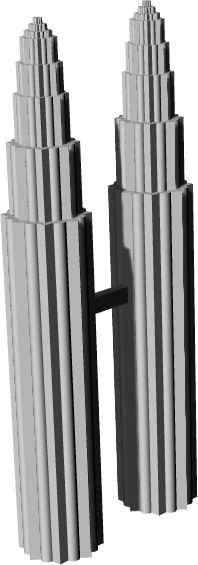
\includegraphics[height=3cm]{fig/case-study-petronas}}
  \hfill
  \subcaptionbox{Voronoi cage.\label{fig:eval.studies.designs.watercube}}
    [.65\linewidth]{%
      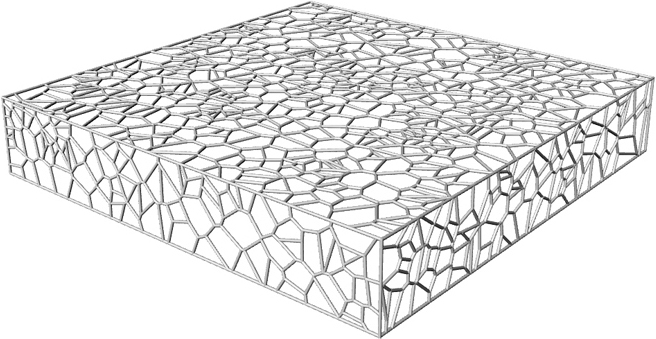
\includegraphics[width=\linewidth]{fig/case-study-water-cube}}
  \caption{\label{fig:eval.studies.designs}
    Case study designs inspired by César Pelli's Petronas Twin
    Towers~\subref{fig:eval.studies.designs.petronas}, and PTW Architects'
    Beijing National Aquatics
    Center~\subref{fig:eval.studies.designs.watercube}.}%
\end{figure}

\subsubsection{Star with Semicircles}%
\label{sec:eval.studies.star}

The first case study is a star shape with semicircles, inspired by César Pelli's
Petronas tower floor plan.  The contour of the Petronas tower floor plan is
formed by two overlapping congruent squares, forming an octagram, and by eight
circles each centered on one of the eight intersection points and tangent to the
bounding octagon.  This shape can be generalized to a parametric shape, shown in
(\cref{fig:eval.studies.star.prob.params}).  Variations are illustrated in
\cref{fig:eval.studies.star.prob}.

\begin{figure}[htb]
  \centering
  \subcaptionbox{\label{fig:eval.studies.star.prob.params}%
    Parametrization.}
    {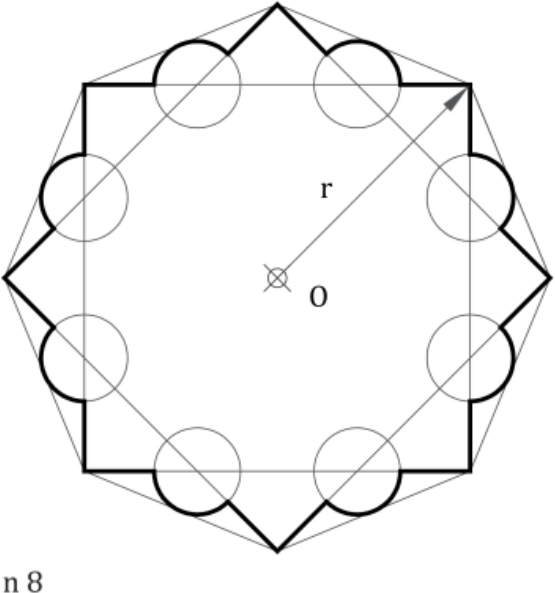
\includegraphics[width=.45\linewidth]{fig/star-problem-params}}
  \hfill
  \subcaptionbox{\label{fig:eval.studies.star.prob.vars}%
    Shape variations.}
    {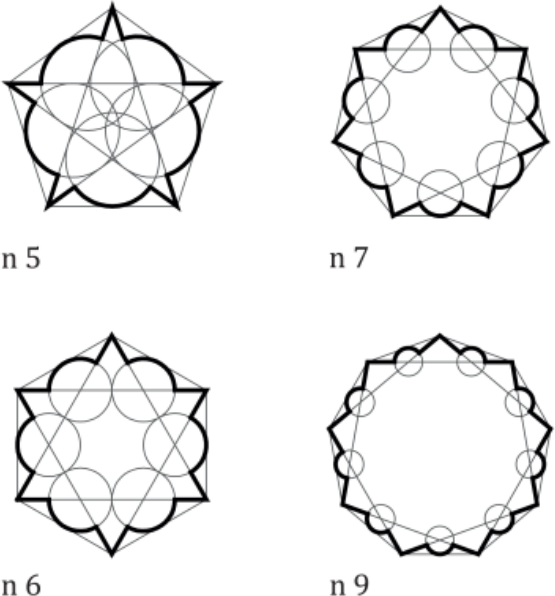
\includegraphics[width=.45\linewidth]{fig/star-problem-vars}}
  \caption{\label{fig:eval.studies.star.prob}
    Star with semicircles problem: \subref{fig:eval.studies.star.prob.params}
    shows our parametrization of the star which can be used to generate shape
    variations, some of them shown in
    \subref{fig:eval.studies.star.prob.vars}.}%
\end{figure}

Both analytic and constructive solutions are based on computing one side of the
star, composed of the line segment $\overline{V_1 I_1}$, the arc centered on
$O_1$ from $I_1$ to $I_2$, with radius $r_1$, and the line segment 
$\overline{I_2 V_2}$ (\cref{fig:eval.studies.star.sol}).

\begin{figure}[htb]
  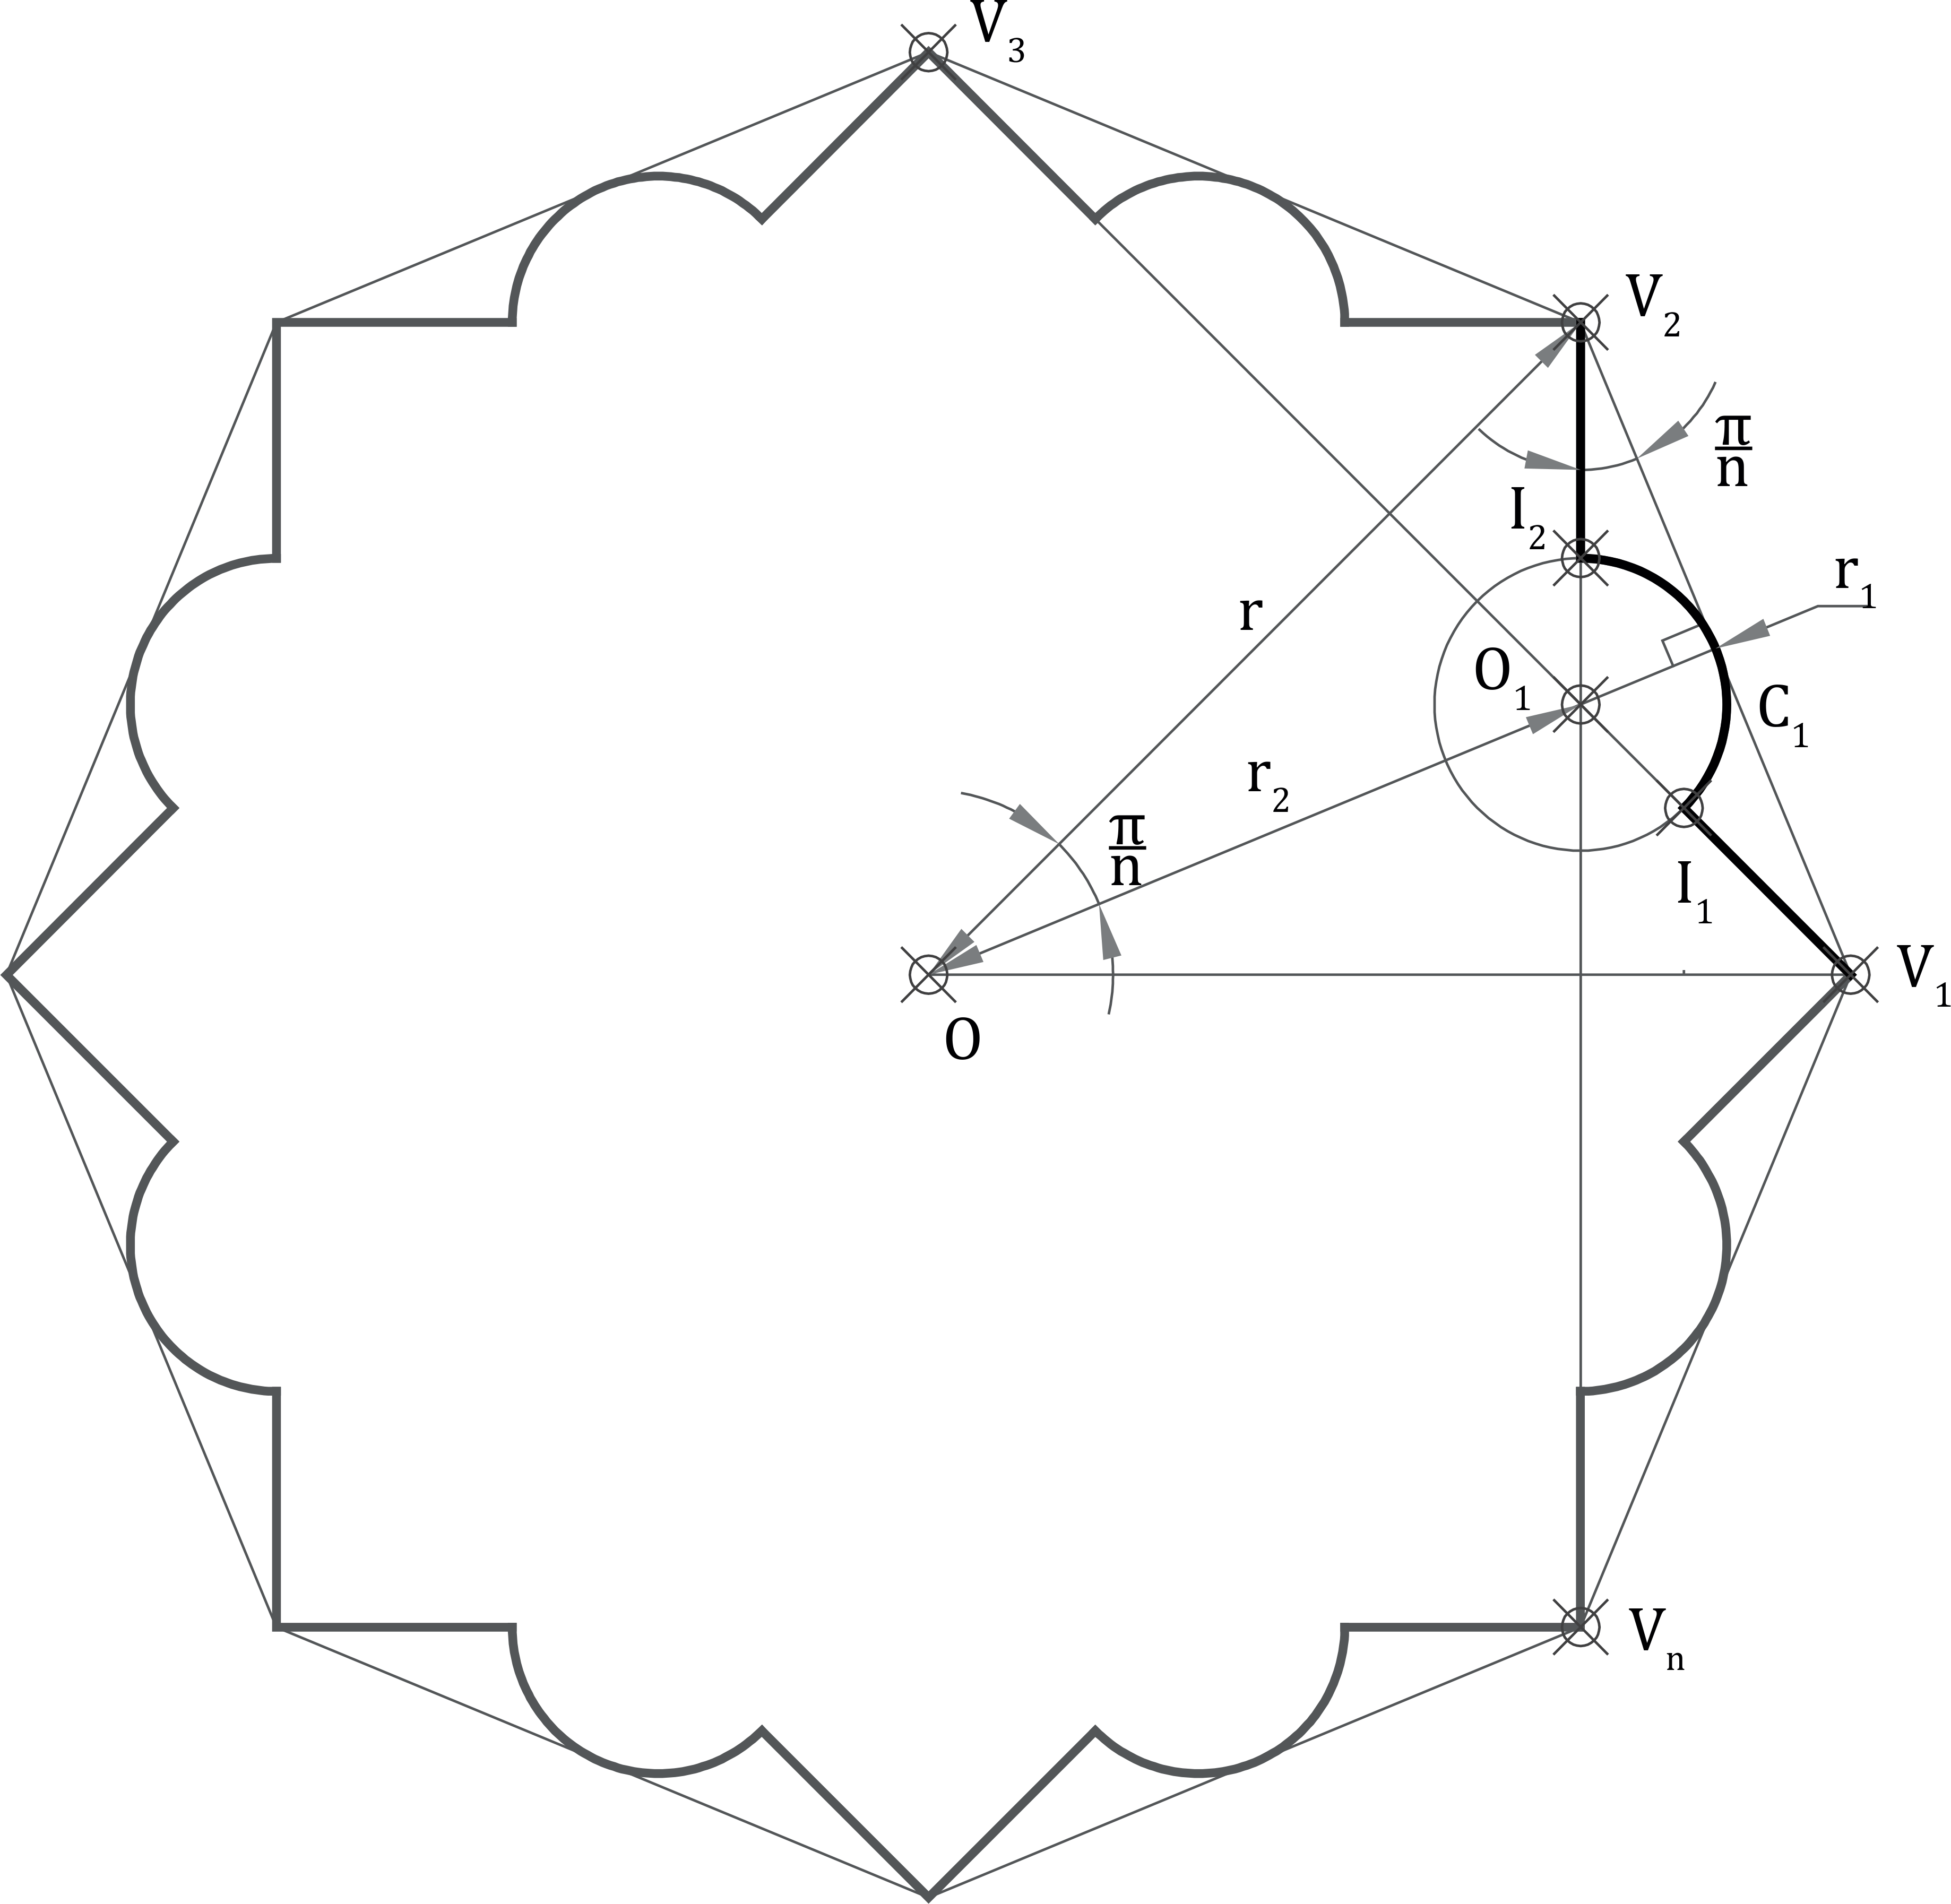
\includegraphics[width=.7\linewidth]{fig/star-solution}
  \caption{\label{fig:eval.studies.star.sol}
    Analytic and constructive solutions to the star with semicircles problem.}%
\end{figure}

The \textit{analytic solution} is described below.

\begin{enumerate}
  \item $r_1 = r\frac{\sin^2\frac{\pi}{n}}{\cos\frac{\pi}{n}}$
  \item $r_2 = r\cos\frac{\pi}{n} - r_1$
  \item $O_1 = O + \left(r_2, \angle\frac{\pi}{n}\right)$
  \item $I_1 = O_1 + \left(r_1, \angle\frac{2\pi}{n} - \frac{\pi}{2}\right)$
  \item $I_2 = O_1 + \left(r_1, \angle\frac{\pi}{2}\right)$
\end{enumerate}

The \textit{constructive solution} is described below.  It uses two primitives
from our solution, namely \texttt{intersection} and \texttt{tangent\_circle}.

\begin{enumerate}
  \item $O_1 = \operatorname{intersection}\left(\overline{V_1 V_3},
  \overline{V_2 V_n}\right)$
  \item $C_1 = \operatorname{tangent_{circle}}\left(O_1, \overline{V_1
  V_2}\right)$
  \item $P,r_1 = C_1$
  \item $I_1 = \operatorname{intersection}\left(\overline{V_1 V_3}, C_1\right)$
  \item $I_2 = \operatorname{intersection}\left(\overline{V_2 V_n}, C_1\right)$
\end{enumerate}

Achieving the equations in the \textit{analytic solution} is not a
straightforward task. It is also unclear how those equations were derived. By
contrast, in the \textit{constructive solution}, all the steps are clearly
externalized, which makes it much easier to understand.

\subsubsection{Voronoi Diagram}%
\label{sec:eval.studies.voronoi}

Our second case study is that of Voronoi diagrams, which are used in a variety
of design fields.  For instance, several facade designs exhibit a Voronoi
appearance, such as PTW Architects' Beijing National Aquatics Center.

\Cref{fig:eval.studies.voronoi.prob} shows three Voronoi diagrams generated from
entirely randomly distributed points, from random points with one attractor
point, and from random points with one attractor line.

\begin{figure}[htb]
  \subcaptionbox{\label{fig:eval.studies.voronoi.prob.rand}}
    {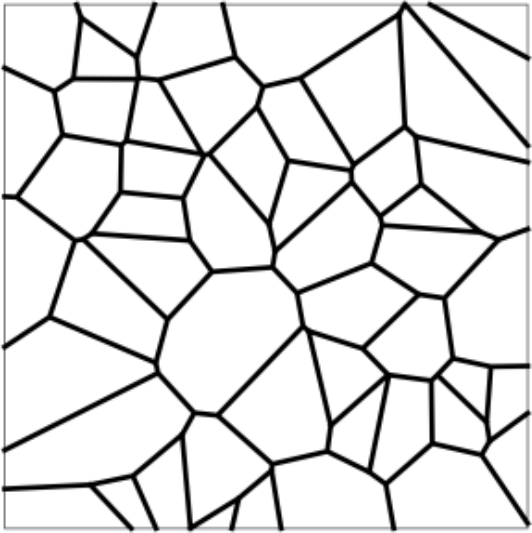
\includegraphics[width=.3\linewidth]{fig/voronoi-problem-rand}}
  \hfill
  \subcaptionbox{\label{fig:eval.studies.voronoi.prob.1attr}}
    {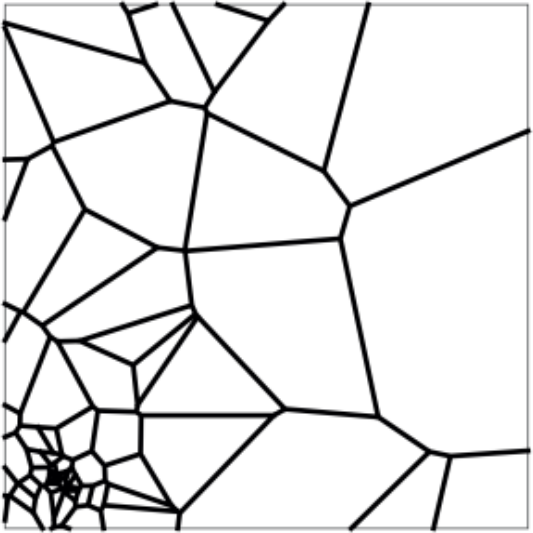
\includegraphics[width=.3\linewidth]{fig/voronoi-problem-1attr}}
  \hfill
  \subcaptionbox{\label{fig:eval.studies.voronoi.prob.edge}}
    {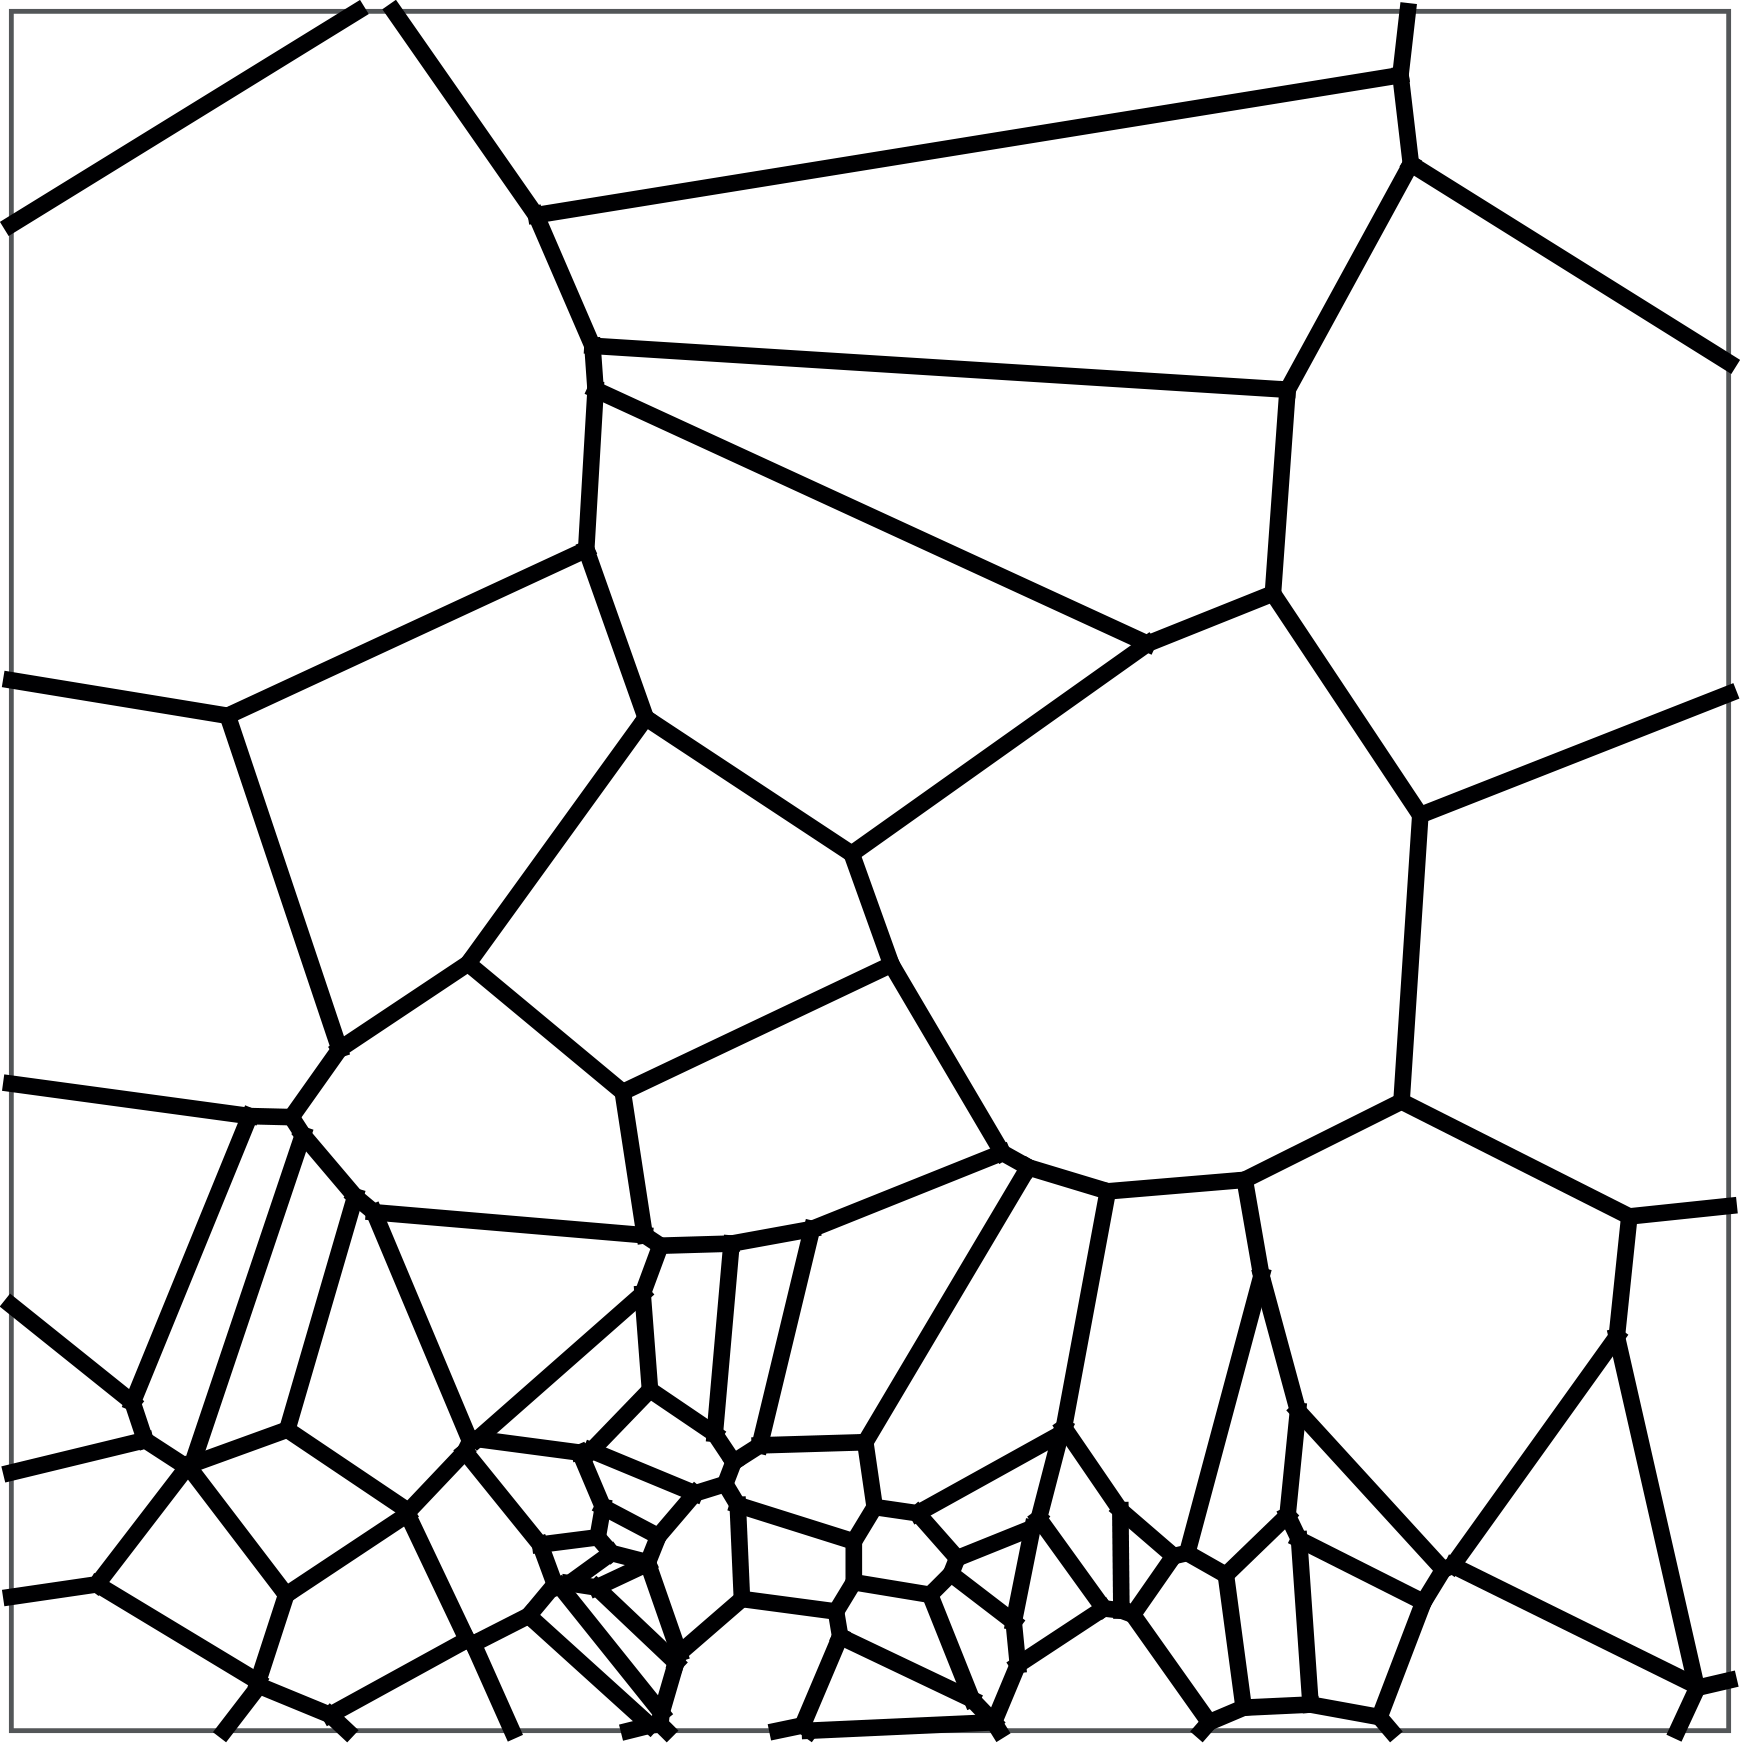
\includegraphics[width=.3\linewidth]{fig/voronoi-problem-edge}}
  \caption[Voronoi diagram problem]{
    Voronoi diagram problem: \subref{fig:eval.studies.voronoi.prob.rand} is
    entirely random, \subref{fig:eval.studies.voronoi.prob.1attr} adds an
    attractor point, and \subref{fig:eval.studies.voronoi.prob.edge} adds an
    attractor line.}%
  \label{fig:eval.studies.voronoi.prob}
\end{figure}

Both the analytic and constructive methods focus on computation of a vertex
relies on the computation of the \textit{circumcenter} of a triangle, for
instance, triangle $\triangle P_1 P_2 P_3$
(\cref{fig:eval.studies.voronoi.sol}).

\begin{figure}[htb]
  \centering
  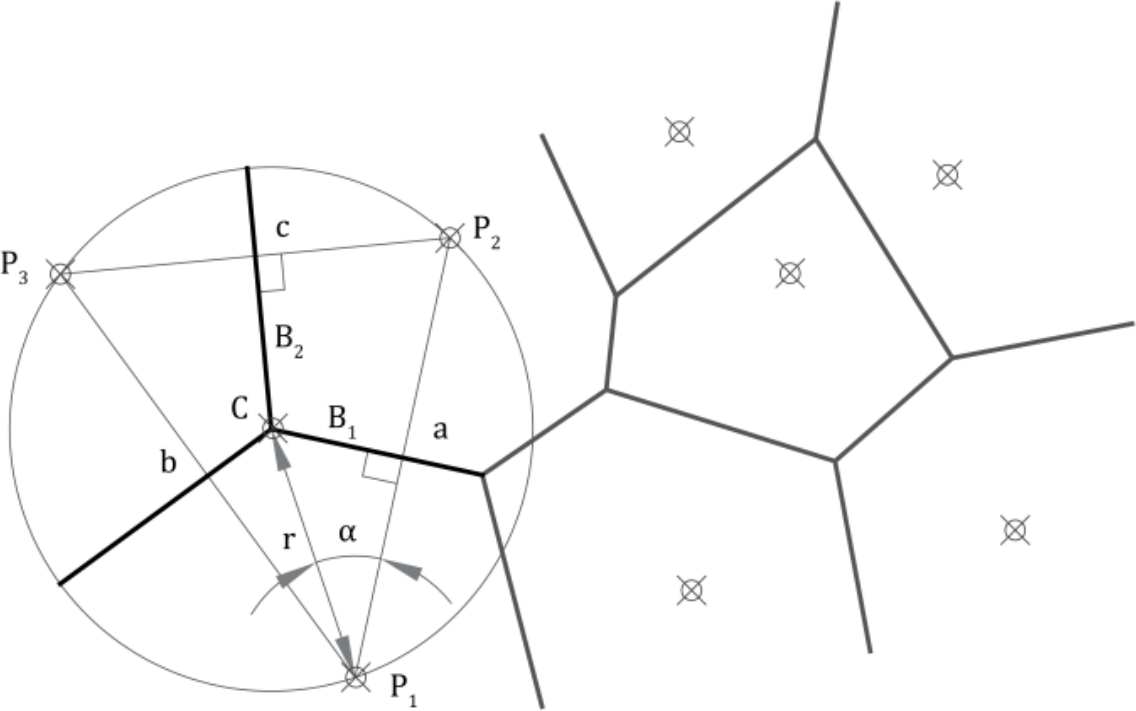
\includegraphics[width=.7\linewidth]{fig/voronoi-solution}
  \caption{\label{fig:eval.studies.voronoi.sol}
    Analytic and constructive approaches to computing a Voronoi vertex.}%
\end{figure}

One possible \textit{analytic solution} is based on the \textit{circumradius}
formula.  The circumcenter $C$ can then be easily computed by a translation from
$P_1$ following the angle $\alpha$.

\begin{enumerate}
  \item $a, b, c = \lVert P_2 - P_1 \rVert, \lVert P_3 - P_1 \rVert, \lVert P_3
  - P_2 \rVert$
  \item $s = \frac{a + b + c}{2}$
  \item $A = \sqrt{s(s - a)(s - b)(s - c)}$
  \item $r = \frac{abc}{4A}$
  \item $\alpha = \arccos\frac{a}{2r}$
  \item $C = P_1 + \left(r, \angle\alpha\right)$
\end{enumerate}

The \textit{constructive solution} computes the circumcenter, directly provided
by our \primitives{}.

\begin{itemize}
  \item[] $C = \operatorname{circumcenter}\left(P_1, P_2, P_3\right)$
\end{itemize}

The circumcenter is only a sub-problem of the generation of a Voronoi diagram.
We first need to build a Delaunay triangulation.  Then, we can apply the
\texttt{circumcenter} to find the Voronoi vertices and draw the diagram's edges.

Implementing this functionality from scratch is a demanding and error-prone
task.  Fortunately, \ac{CGAL} already has an algorithm that produces Voronoi
diagrams.  This algorithm was made available in \texttt{CGAL.jl},
and, thus, it is also available in our solution.  The final section of the
evaluation goes over how we can repurpose this algorithm as a side effect of
integrating such a comprehensive library as \ac{CGAL}.
